\chapter{\textbf{Parameterization}}

In order to have a mapping beetwen the consumption of our Physical Resources and Virtual Resources we identified a Overhead Matrix:

\begin{center}
\makebox[\textwidth]{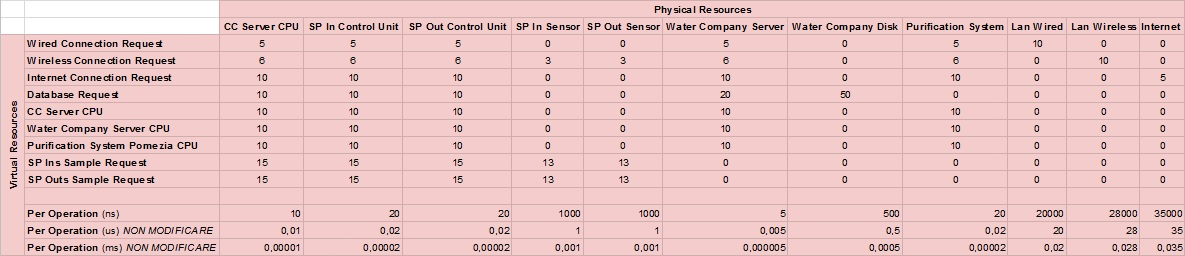
\includegraphics[width=\textwidth]
{1-OverheadMatrix.jpg}}
\end{center}
\captionof{figure}{Overhead Matrix}
\bigskip

In the last three rows of the table are specified the service time for Physical Resources to execute a basic operation.\\
The next step is obtain the whole consumption of our Virtual Resources for each Execution Graph considering the meaning of each individual block:

\begin{center}
\makebox[\textwidth]{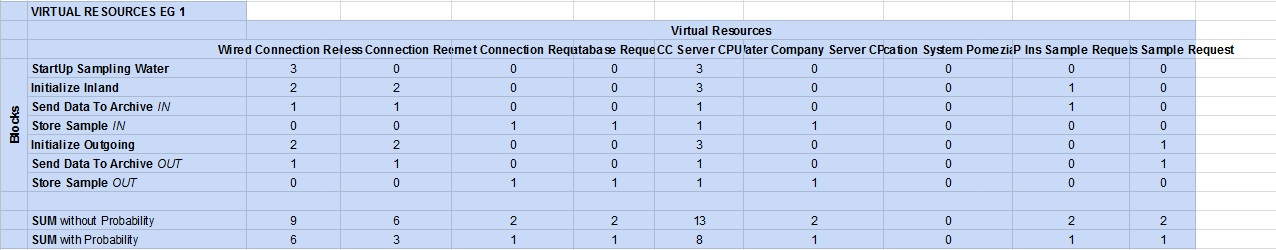
\includegraphics[width=\textwidth]
{2-VirtualResUsagebyeachNode.jpg}}
\end{center}
\captionof{figure}{Virtual Resource Usage By Each Block}


\begin{center}
\makebox[\textwidth]{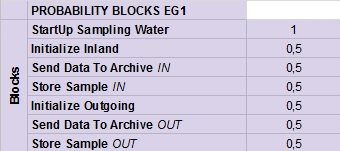
\includegraphics[width=7cm]
{3-Probeachnode.jpg}}
\end{center}
\captionof{figure}{Block Probability}
\bigskip

Considering this last table with the overhead matrix we obtain a matrix containing the consumption of the physical resources related to the considered Execution Graph. This method was applied for both execution graphs and then we reapplied it once we decided to split the jobs.

\begin{center}
\makebox[\textwidth]{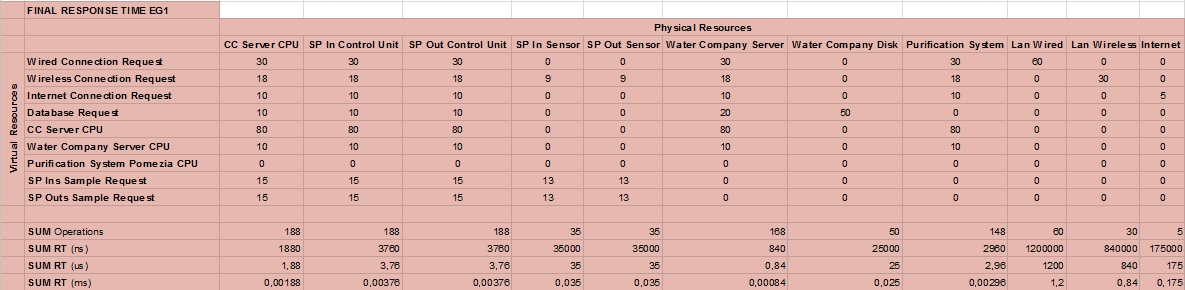
\includegraphics[width=\textwidth]
{4-FinalRes.jpg}}
\end{center}
\captionof{figure}{Final Resources Consumption}

Having introduced two differnt classes of jobs, for the same reasons expressed in the chapter 8, wh have also to re-evaluate the service demand of the new classes of jobs. 
For more details we refer to the attached excel files.
